\documentclass[8pt,a4paper,compress]{beamer}

\usepackage{/home/siyer/lib/slides}

\title{Programming Environment}
\date{}

\newlength{\myMheight}
\settoheight{\myMheight}{M}

\begin{document}
\begin{frame}
\vfill
\titlepage
\end{frame}

\section{Programming Environment}
\begin{frame}[fragile]
\pause\transdissolve

VirtualBox

\pause\transdissolve\bigskip

Linux-based virtual machine (ElementaryOS)

\pause\transdissolve\bigskip

\begin{center}
\visible<4->{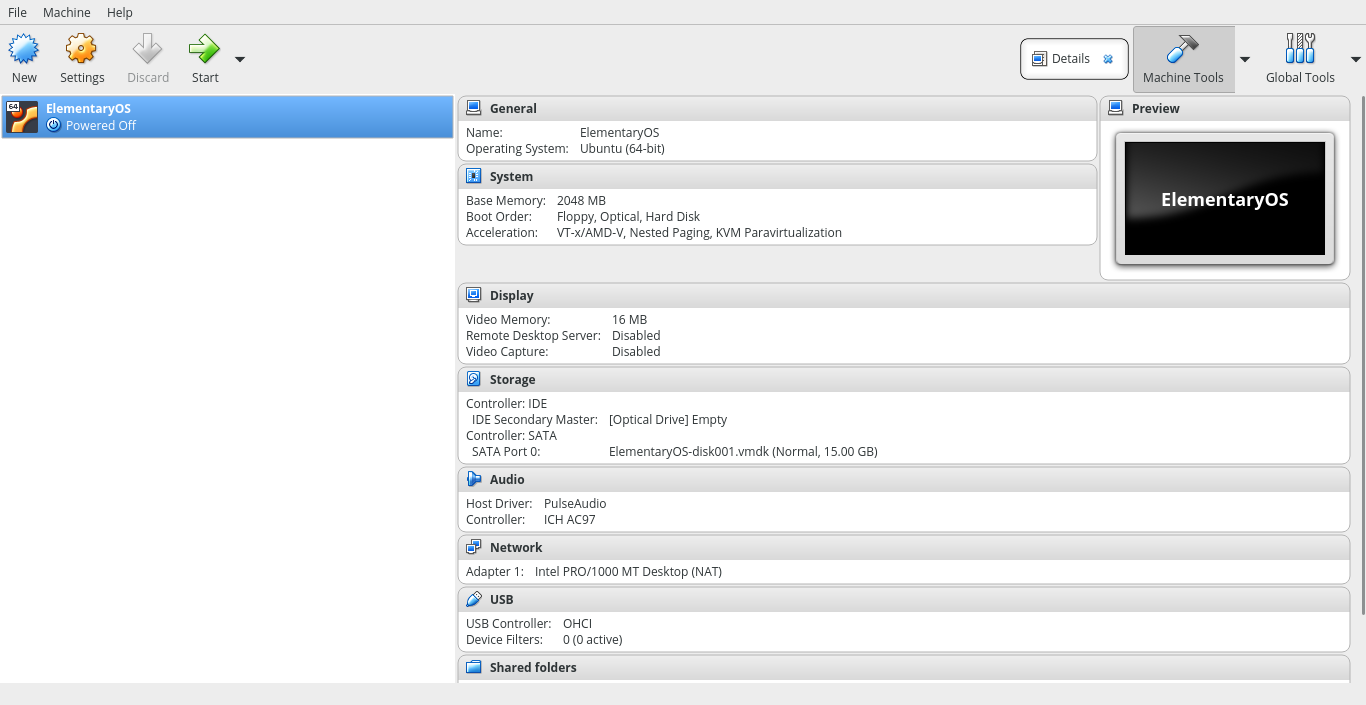
\includegraphics[scale=0.2]{figures/vbox.png}}
\end{center}
\end{frame}

\section{ElementaryOS}
\begin{frame}[fragile]
\pause\transdissolve

Click ``Start'' to start the machine

\pause\transdissolve\bigskip

Login as Uber Student (username \lstinline{student}) with password \lstinline{enigma}

\pause\transdissolve\bigskip

\begin{center}
\visible<4->{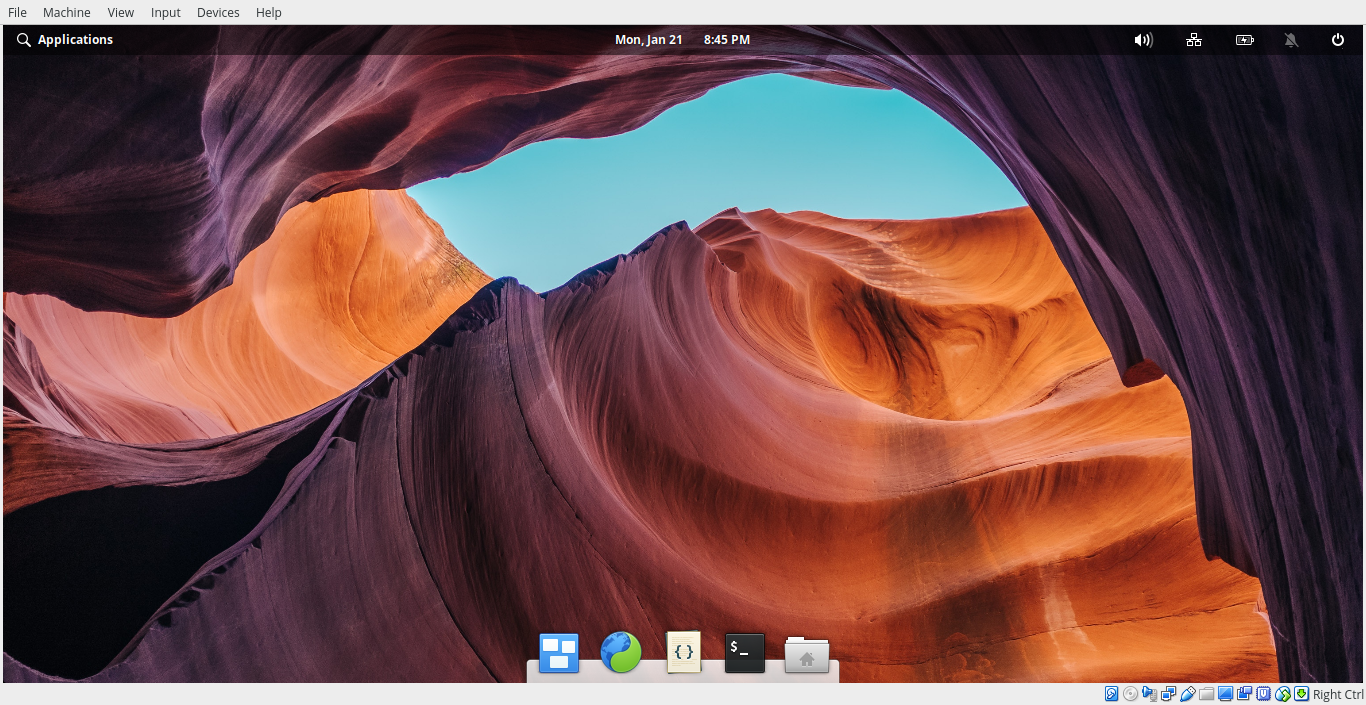
\includegraphics[scale=0.2]{figures/elementaryos.png}}
\end{center}

\pause\transdissolve\bigskip

To stop the machine, click \visible<5->{
\includegraphics[height=\myMheight]{figures/shutdown.pdf}} and select ``Shut Down...''
\end{frame}

\section{Tools}
\begin{frame}[fragile]
\pause\transdissolve

Web browser \visible<2->{
\includegraphics[height=\myMheight]{figures/web_browser.pdf}}

\pause\transdissolve\bigskip

Editor \visible<3->{
\includegraphics[height=\myMheight]{figures/editor.pdf}}

\pause\transdissolve\bigskip

Terminal \visible<4->{
\includegraphics[height=\myMheight]{figures/terminal.pdf}}

\pause\transdissolve\bigskip

File manager \visible<5->{
\includegraphics[height=\myMheight]{figures/file_manager.pdf}}
\end{frame}

\section{Editing Files}
\begin{frame}[fragile]
\pause\transdissolve

Use editor \visible<2->{
\includegraphics[height=\myMheight]{figures/editor.pdf}}

\smallskip

\begin{center}
\visible<2->{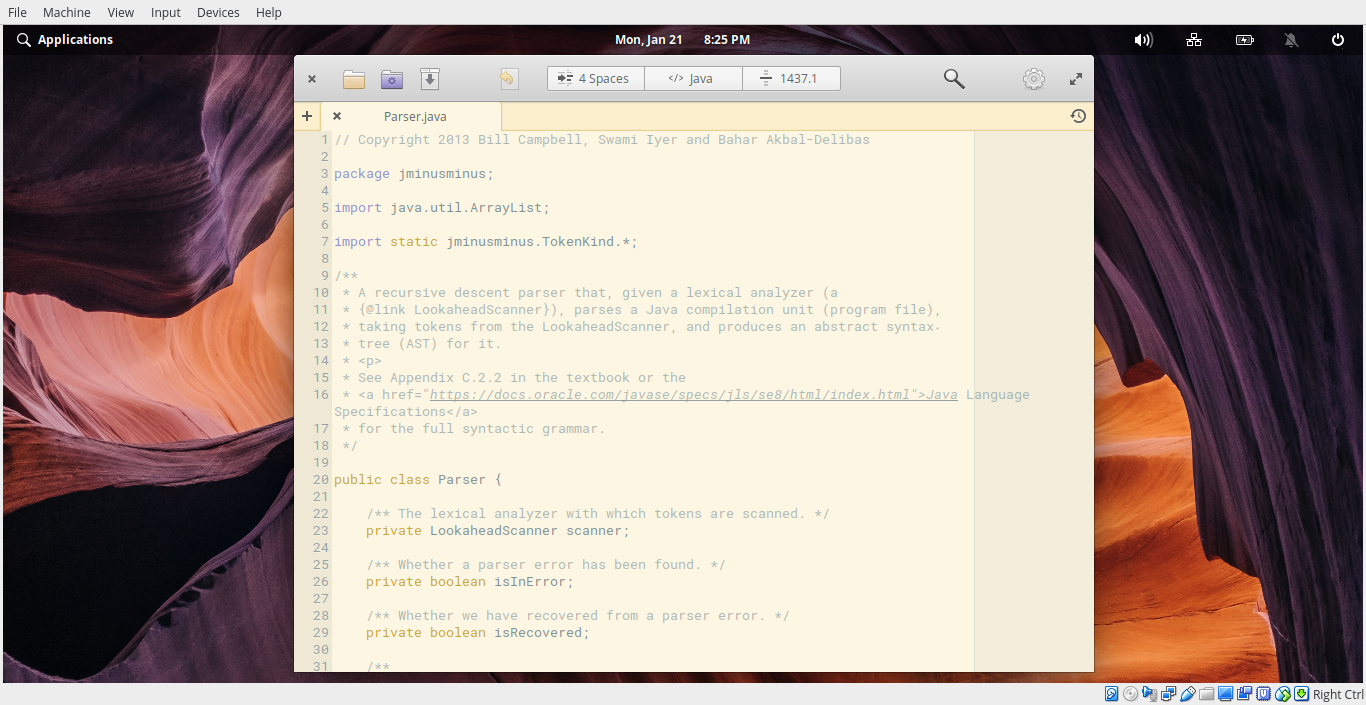
\includegraphics[scale=0.2]{figures/editing.png}}
\end{center}
\end{frame}

\section{Navigating the File System}
\begin{frame}[fragile]
\pause\transdissolve

Use file manager \visible<2->{
\includegraphics[height=\myMheight]{figures/file_manager.pdf}} and terminal \visible<2->{
\includegraphics[height=\myMheight]{figures/terminal.pdf}}

\smallskip

\begin{center}
\visible<2->{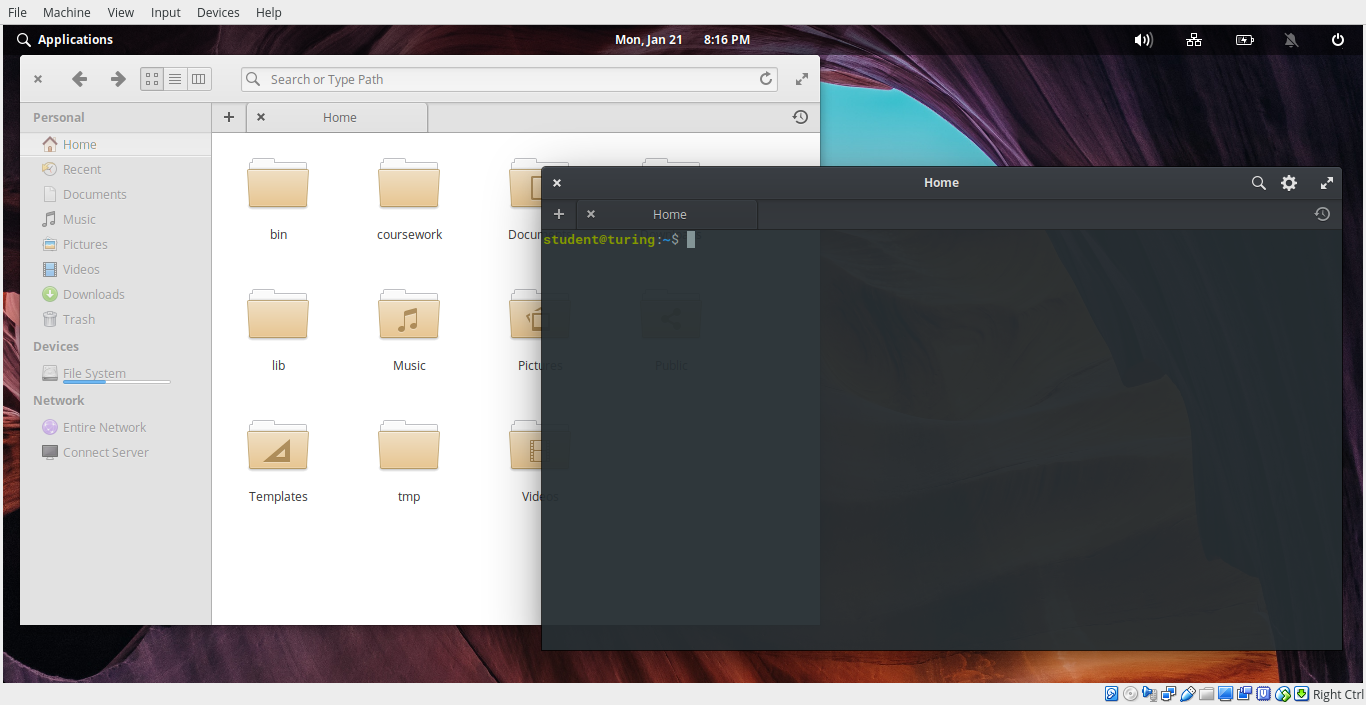
\includegraphics[scale=0.2]{figures/filesystem.png}}
\end{center}
\end{frame}

\section{Obtaining the Base \protect \jmm Compiler}
\begin{frame}[fragile]
\pause\transdissolve

Launch terminal (opens in \lstinline{/home/student} by default)

\pause\transdissolve\bigskip

Change directory to \lstinline{coursework}

\begin{tcolorbox}[enhanced,drop shadow southwest,sharp corners,size=fbox,colback=black]
\begin{lstlisting}[style=terminal]
$ cd coursework
\end{lstlisting}
\end{tcolorbox}

\pause\transdissolve\bigskip

Download the base \jmm compiler

\begin{tcolorbox}[enhanced,drop shadow southwest,sharp corners,size=fbox,colback=black]
\begin{lstlisting}[style=terminal]
$ wget https://swamiiyer.net/cs451/j--.zip
\end{lstlisting}
\end{tcolorbox}

\pause\transdissolve\bigskip

Extract the downloaded zip file

\begin{tcolorbox}[enhanced,drop shadow southwest,sharp corners,size=fbox,colback=black]
\begin{lstlisting}[style=terminal]
$ unzip j--.zip
\end{lstlisting}
\end{tcolorbox}

\pause\transdissolve\bigskip

Remove the zip file

\begin{tcolorbox}[enhanced,drop shadow southwest,sharp corners,size=fbox,colback=black]
\begin{lstlisting}[style=terminal]
$ rm j--.zip
\end{lstlisting}
\end{tcolorbox}
\end{frame}

\section{Working with the \protect \jmm Compiler}
\begin{frame}[fragile]
\pause\transdissolve

Change directory to \lstinline{j--}

\begin{tcolorbox}[enhanced,drop shadow southwest,sharp corners,size=fbox,colback=black]
\begin{lstlisting}[style=terminal]
$ cd j--
\end{lstlisting}
\end{tcolorbox}

\pause\transdissolve\bigskip

We are now under \lstinline{/home/student/coursework/j--}, which we refer to as \lstinline{$j}

\pause\transdissolve\bigskip

Compile the \jmm compiler

\begin{tcolorbox}[enhanced,drop shadow southwest,sharp corners,size=fbox,colback=black]
\begin{lstlisting}[style=terminal]
$ ant
\end{lstlisting}
\end{tcolorbox}

\pause\transdissolve\bigskip

Compile the \jmm program \lstinline{$j/tests/pass/HelloWorld.java} for the JVM architecture

\begin{tcolorbox}[enhanced,drop shadow southwest,sharp corners,size=fbox,colback=black]
\begin{lstlisting}[style=terminal]
$ sh ./bin/j-- tests/pass/HelloWorld.java
\end{lstlisting}
\end{tcolorbox}

\pause\transdissolve\bigskip

Run the JVM program \lstinline{HelloWorld.class}

\begin{tcolorbox}[enhanced,drop shadow southwest,sharp corners,size=fbox,colback=black]
\begin{lstlisting}[style=terminal]
$ java pass.HelloWorld
\end{lstlisting}
\end{tcolorbox}

\pause\transdissolve\bigskip

Disassemble \lstinline{HelloWorld.class}

\begin{tcolorbox}[enhanced,drop shadow southwest,sharp corners,size=fbox,colback=black]
\begin{lstlisting}[style=terminal]
$ javap -p -v pass.HelloWorld
\end{lstlisting}
\end{tcolorbox}
\end{frame}

\begin{frame}[fragile]
\pause\transdissolve

Compile the \jmm program \lstinline{$j/tests/spim/HelloWorld.java} for the MIPS architecture

\begin{tcolorbox}[enhanced,drop shadow southwest,sharp corners,size=fbox,colback=black]
\begin{lstlisting}[style=terminal]
$ sh ./bin/j-- -s naive tests/spim/HelloWorld.java
\end{lstlisting}
\end{tcolorbox}

\pause\transdissolve\bigskip

Run the MIPS program \lstinline{HelloWorld.s}

\begin{tcolorbox}[enhanced,drop shadow southwest,sharp corners,size=fbox,colback=black]
\begin{lstlisting}[style=terminal]
$ spim -f HelloWorld.s
\end{lstlisting}
\end{tcolorbox}

\pause\transdissolve\bigskip

Create file \lstinline{j--.tar.gz} for submission on Gradescope

\begin{tcolorbox}[enhanced,drop shadow southwest,sharp corners,size=fbox,colback=black]
\begin{lstlisting}[style=terminal]
$ ant clean
$ cd ..
$ tar -cvf j--.tar j--/*
$ gzip j--.tar
\end{lstlisting}
\end{tcolorbox}

\pause\transdissolve\bigskip

Use web browser \visible<5->{
\includegraphics[height=\myMheight]{figures/web_browser.pdf}} to sign on to Gradescope and upload your project files
\end{frame}
\end{document}
